\documentclass[12pt]{article}
\usepackage[margin=0.5in]{geometry} 
\usepackage{amsmath,amsthm,amssymb,amsfonts, enumitem, fancyhdr, color, comment, graphicx, environ}
\usepackage{course}
\usepackage{cse468-Spring23}
\usepackage{program}
\usepackage{fancybox}
\usepackage{adjustbox}
\usepackage{quantikz}
\usepackage{../bbkey}
\def\SquareOutline{%
\path (0,0) rectangle (1,1);%
}%
\def\Gate#1{\mbox{\textbf{#1}}}
\def\X{\Gate{X}}
\def\Z{\Gate{Z}}
\def\I{\Gate{I}}
\def\H{\Gate{H}}
\def\QZero{\ket{0}}
\def\QState#1{\ensuremath{\psi_{#1}}}

\def\Obox#1{\Ovalbox{\hbox to 1ex{\vrule width 0pt height 1ex\hss #1\hss}}}
\def\TFMarked#1#2{\ \stackbox[l][m]{\Obox{#1}~\textbf{true}\\\Obox{#2}~\textbf{false}}}
\def\TF{\TFMarked{\relax}{\relax}}
\def\exp#1{\ensuremath{e^{#1}}}
\newcommand{\Blank}[1][1in]{\mbox{\vrule width #1 depth 2pt}\vrule width 0pt height 2.0em}
\def\BlQb{\mbox{\ensuremath{\Blank[4em]\ket{0}+\Blank[4em]\ket{1}}}}
\newcommand{\Blanket}[1][3em]{%
\mbox{\ensuremath{|\,\Blank[#1]\,\rangle}}}

\def\Tall{\vrule width 0pt height 2em depth 0.5em}

\def\SQB#1#2{%
\ensuremath{%
\begin{pmatrix*}[r] #1 \\ #2\end{pmatrix*}}}

\def\SQBB{\SQB{\Blank[2em]}{\Blank[2em]}}

\def\DQB#1#2#3#4{%
\ensuremath{%
\begin{pmatrix*}[r] #1 \\ #2 \\ #3 \\ #4\end{pmatrix*}}}
\def\DQBB{\DQB{\Blank[2em]}{\Blank[2em]}{\Blank[2em]}{\Blank[2em]}}

\def\FactorProof{%
\begin{align*}
\SQB{a}{b} \otimes \SQB{c}{d} &= \DQBB{} \mbox{ (copy this from your \QState{2} answer top of page)}\\
a\cdot c &= \Blank[3em] \\
a\cdot d &= \Blank[3em] \\
b\cdot c &= \Blank[3em] \\
b\cdot d &= \Blank[3em]
\end{align*}
What is the contradiction, if any?
\LeaveSpace{2in}
}

\begin{document}

\begin{assignment}{Exam II}{26 April 2023}{End of class}

{\small {\large \fbox{READ THIS before starting!}}
This exam is open-book, open-notes, open-Internet, but you must do this
work on your own without contact or conversations with any person.
Because this exam is given in a somewhat distributed manner, no questions will be answered, and no clarifications will be given.  State your assumptions and count on us to be fair and flexible, especially if we have been unclear.


Your work must be legible.  Work that is
difficult to read will receive no credit.  There is a blank page at the end
if you want to show extra work there.

There are 116 points available for this exam, but it will only be scored out of 100.  Extra points earned here will count toward your total exam grade.

You must sign the pledge below for your exam to count.  Any cheating will
cause the students involved to receive an F for this course. Other unpleasant
actions
may be taken.

You must fill in your identifying information correctly.  
}

\begin{center}\large
\begin{tabular}{|c|c|c|} \hline
\multicolumn{3}{|c|}{{\bf Print  clearly} the following information:}  \\ \hline
\multicolumn{3}{|l|}{Name (print clearly):\Tall{}\hbox to 3in{\hss}}  \\ \hline
\multicolumn{3}{|l|}{Student 6-digit ID (print {\it really} clearly):\Tall{}\hbox to 3in{\hss}} \\ \hline
\end{tabular}
\end{center}

{\bf Pledge:} On my honor, I have neither
given nor received any unauthorized aid on this exam.

Signed:  \Blank\Blank\Blank\Blank \\ \hbox to 5em{\hss}(Be 
sure you filled in your information in the box above!)
%
%
%
\clearpage
\begin{enumerate}
\item\Points{30} For the \textbf{true}/\textbf{false} questions below, indicate your response by marking an~\textbf{x} in the appropriate box, like this:
\TFMarked{\textbf{x}}{\relax} or \TFMarked{\relax}{\textbf{x}}.  

Each response is worth 3 points and there are 6 points of extra credit available here.
\begin{itemize}
    \item Deutsch--Jozsa solves a problem in polynomial time on a quantum computer that takes worst-case exponential time on a classical computer.~\TF{}
    \item With a single query, a classical computer has at least a 50\% chance of determining the correct solution to a Deutsch--Jozsa problem.~\TF{}
    \item An $n$-bit instance of Bernstein--Vazirani can take $\Theta(2^{n})$ time on a classical computer to solve exactly.~\TF{}
    \item An $n$-bit instance of Simon's problem can take $\Theta(2^{n})$ time on a classical computer to solve exactly.~\TF{}
    \item If the Deutsch--Jozsa quantum algorithm is presented with an oracle from Bernstein--Vazirani with secret $s$, then the circuit's measurements will yield a unique result (depends only on $s$) in the computational basis.~\TF{}
    \item If the entangled qubits for the CHSH game fail (they decohere and collapse into random values), Alice and Bob can at best win 75\% of the time.~\TF{}
    \item In the Mermin--Peres square, each of Alice's qubits is entangled with one of Bob's qubits.  If that entanglement did not exist, the values Alice reports for her assigned rows still multiply to $+1$, as they should.~\TF{}
    \item In the Mermin--Peres square, each of Alice's qubits is entangled with one of Bob's qubits.  If that entanglement did not exist, Alice and Bob would still agree on the value of their shared square, as they should.~\TF{}
    \item Grover's algorithm provides exponential speedup over classical algorithms that solve the same problem.~\TF{}
    \item Shor's algorithm provides exponential speedup over the best-known approach for factoring large integers.~\TF{}
    \item Grover's algorithm can solve the factoring problem as quickly as Shor's algorithm.~\TF{}
    \item The university course evaluation for this course is worth one of the five points for participation in this class.  You agree to complete the evaluation by May~11.~\TF{}
\end{itemize}

\clearpage\item\Points{10} Recall the Mermin--Peres square below.

\begin{tabular}{cc}
\begin{minipage}[t]{2.8in}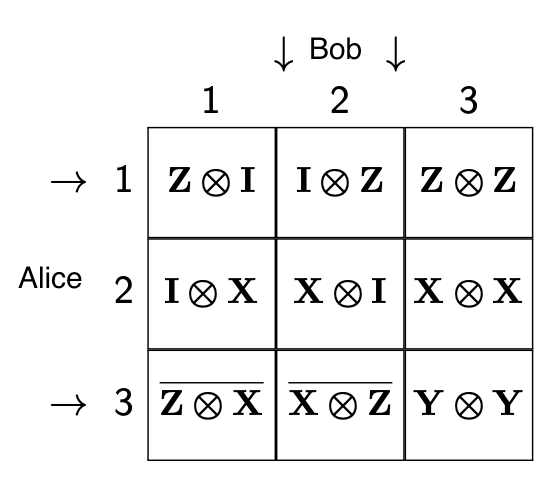
\includegraphics[scale=0.6]{mp.png}\end{minipage} &
\raisebox{1.2in}{\begin{minipage}[t]{3in}\raggedright Alice, having traveled to Israel, decides to compute her squares' results \textbf{right to left}, while Bob, still in St.~Louis, reports his results top to bottom, as usual.\end{minipage}}
\end{tabular}

\begin{enumerate}

\item\Points{2} With this change to Mermin--Peres, answer the following questions:

\begin{itemize}
    \item For any of her three rows, Alice \emph{always} reports values whose products are $+1$ as required.~\TF{}
    \item Alice and Bob \emph{always} agree on a value in their common square.~\TF{}

\end{itemize}
\item\Points{4} Below, explain your answers to part~(a), by providing an example that makes a statement false, or by explaining why the statement is true.
    \LeaveSpace{2in}

\item\Points{4} Suppose Alice happens to measure first, measuring $\ket{++}$ for her $\X{}\otimes\X{}$ square.

Fill in the blanks below showing \emph{all possible values} that could be reported following Alice's measurement.

\medskip

\begin{tabular}{cc}
\begin{minipage}{3in}
Alice row 2
\begin{itemize}
    \item Right square \Blank[4em]{}
    \item Center square \Blank[4em]{}
    \item Left square \Blank[4em]{}
\end{itemize}
\end{minipage}
&
\begin{minipage}{3in}
Bob column 2
\begin{itemize}
    \item Top square \Blank[4em]{}
    \item Middle square \Blank[4em]{}
    \item Bottom square \Blank[4em]{}
\end{itemize}
\end{minipage}
\end{tabular}
\end{enumerate}

\clearpage\item\Points{10}

\begin{center}
\begin{minipage}[t]{2.8in}
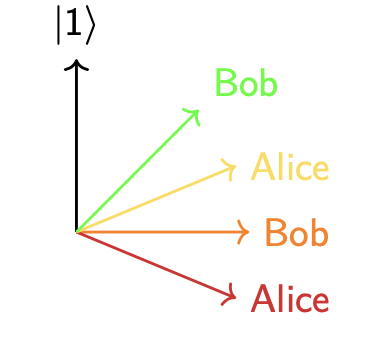
\includegraphics[scale=0.6]{chsh.png}\end{minipage}\end{center}


\begin{itemize}
\item Recall that in the CHSH solution, the angle between adjacent rays in the picture above is $\pi/8$, so that the probability of agreement where it should happen is approximately~$85\%$.
\item Suppose the angle between each adjacent pair of rays is changed to $\pi/16$, so that when they should agree, their probability of agreement is now
\[ \cos^{2}(\pi/16) \approx 96\% \]
\end{itemize}

All other aspects of the game are unchanged:  
\begin{itemize}
    \item Alice and Bob are provided colors that are chosen randomly and uniformly.
    \item The metric for success of the game is the \emph{average} rate at which Alice and Bob agree when they should and disagree when they should, over all 4 possible combinations of colors they can be provided. 
    \item In the original game, as taught, the success metric is approximately~85\%.
\end{itemize}
Answer the following:
\begin{itemize}
    \item\Points{1} This change improves the success of the game.~\TF{}.
    \item\Points{5} What is the approximate success metric of the game with this change? (provide a numeric answer, such as ``85'' for ``85\%'') \Blank{}\%
    \item\Points{3} Show the math supporting your answers below:
    \LeaveSpace{3in}
\end{itemize}

\clearpage\item\Points{10} For each question below, fill in the blank.  Your answer must appear in the provided blank for proper credit.  Write each response in the provided blank space, fully above the dark line.  For example, to express $\frac{i}{\sqrt{3}}$ you would write \Blank{}\hbox to 0pt{\hskip -4em\raisebox{4pt}{$i/\sqrt{3}$}\hss}.  


\begin{itemize}
    \item Consider the oracle portion of a circuit below for an $8$-bit instance of the Bernstein--Vazirani problem.  Recall the oracle computes $y=x\oplus s$ for a secret bit vector~$s$.
    
    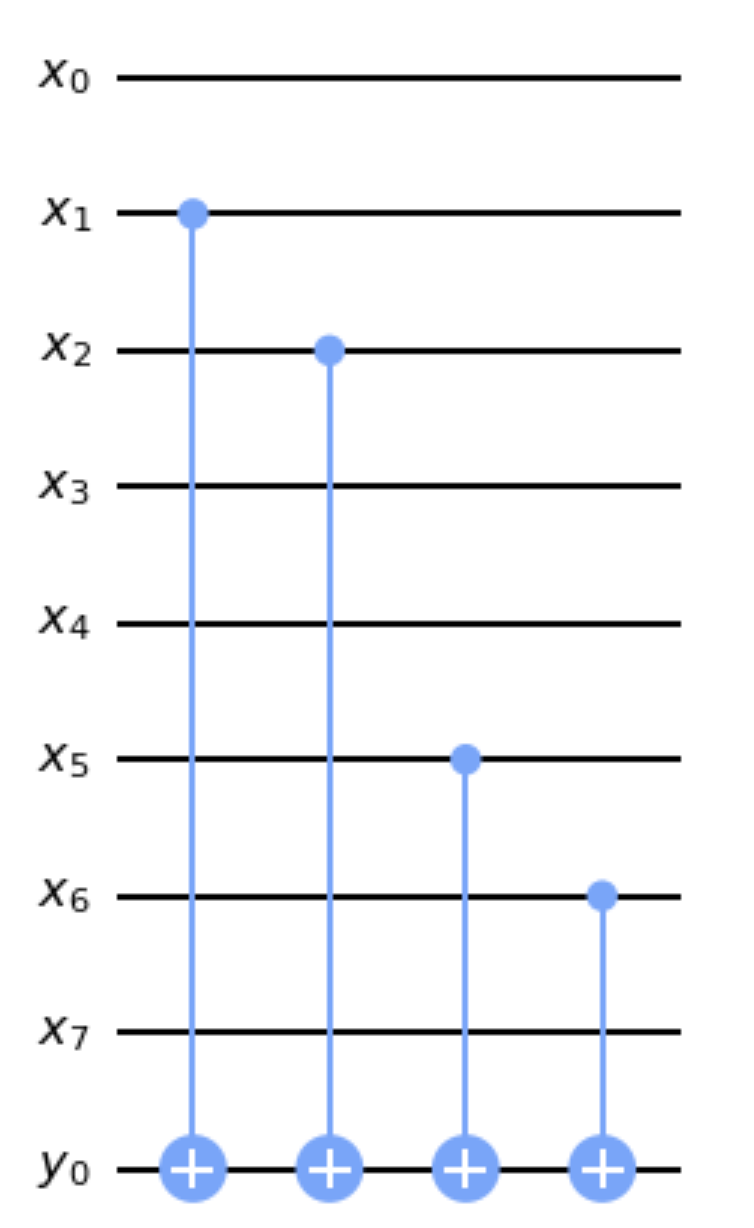
\includegraphics[scale=0.4]{bv.png}
    
    What is the secret $s$ here? \Blank[2in]{}
    \item If this oracle is used in the Deutsch--Jozsa algorithm, what possible amplitude(s) can be measured on $\ket{00000000}$?
    
    \Blank[4in]{}
    \item What other computational basis vector(s), if any, will have non-zero amplitude for Deutsch--Jozsa if the above oracle is used?  
    
    \Blank[4in]{}
\end{itemize}

\clearpage\item\Points{10}
Complete the circuit below so that it is an oracle for Grover's algorithm on a 5-qubit instance, sending $\ket{xy}$ to $\ket{x\ \  y\oplus f(x)}$ where the secret is $10101$.  Below you provide only the oracle, not any other portions of the circuit.

\adjustbox{valign=t,scale=3.0}{\begin{quantikz}
\lstick{$x_1$} &  \qw & \qw & \qw & \qw & \qw\\
\lstick{$x_2$} &  \qw & \qw & \qw & \qw & \qw\\
\lstick{$x_3$} &  \qw & \qw & \qw & \qw & \qw\\
\lstick{$x_4$} &  \qw & \qw & \qw & \qw & \qw\\
\lstick{$x_5$} &  \qw & \qw & \qw & \qw & \qw\\
\lstick{$y$} &  \qw & \qw & \qw & \qw & \qw\\
\end{quantikz}}

\item\Points{5}
Consider a 2-qubit instance of Grover with the secret value $\ket{00}$.  The circuit up to the point of the diffusion step is specified.  Complete the circuit by adding the diffusion (also called reflection about $\ket{s}$) step.

\adjustbox{valign=t,scale=1.3}{\begin{quantikz}
\lstick{$\ket{0}$} & \qw      &  \gate{H} & \gate{X} & \ctrl{2} & \gate{X} & \qw
& \qw & \qw & \qw & \qw & \qw & \qw & \qw & \qw &\qw&\qw\\
\lstick{$\ket{0}$} & \qw      &  \gate{H} & \gate{X} & \ctrl{1} & \gate{X} & \qw& \qw & \qw & \qw & \qw & \qw & \qw & \qw & \qw&\qw&\qw\\
\lstick{$\ket{0}$} & \gate{X} &  \gate{H} & \qw      & \targ{} & \qw & \qw& \qw & \qw & \qw & \qw & \qw & \qw & \qw & \qw&\qw&\qw
\end{quantikz}}

\clearpage\item\Points{10} (1 per blank)
Recall for Grover's problem that when an oracle provided a single secret, we obtained $\ket{w}$ as a column vector of all zeros, but with a 1 in the location of the secret.   For example, for a two-qubit problem ($N=4$) with secret $\ket{00}$ 
\[ \ket{w} = \begin{pmatrix} 1 \\ 0 \\ 0 \\ 0\end{pmatrix} \]
Suppose the oracle instead provides \emph{two} secret values, $\ket{00}$ and $\ket{11}$.  If Grover's algorithm could reach $\ket{w}$ and we performed a measurement of $\ket{w}$ we would be satisfied at measuring \emph{either} secret ($\ket{00}$ or $\ket{11}$).

We begin as before with
\[ \ket{s} = \frac{1}{2}\begin{pmatrix} 1 \\ 1 \\ 1 \\ 1\end{pmatrix} \]

But for this problem with the two secret values $\ket{00}$ and $\ket{11}$ (fill in the blanks):
\[ \ket{w} = \frac{1}{\sqrt{2}}\begin{pmatrix} \Blank[2em]{} \\ \Blank[2em]{} \\\Blank[2em]{} \\\Blank[2em]{} \end{pmatrix} \]
and thus $\ket{s'}$ which must be orthogonal to $\ket{w}$ is (fill in the blanks):
\[ s' = \frac{1}{\sqrt{2}}\begin{pmatrix} \Blank[2em]{} \\ \Blank[2em]{} \\\Blank[2em]{} \\\Blank[2em]{} \end{pmatrix} \]
The inner product of $\ket{s}$ and $\ket{s'}$ is then
\( \braket{s}{s'} = \frac{\Blank[2em]{}}{\sqrt{4}} \) (fill in the numerator)

Generally, for an $n$~qubit instance of Grover ($N=2^n$), where $\ket{w}$ represents $k$ acceptable secret values, what is the inner product of the resulting $\ket{s}$ and $\ket{s'}$? $\frac{\Blank[2em]{}}{\sqrt{N}}$

\Points{5}Complete the circuit below so that it is an oracle for Grover's algorithm on a 2-qubit instance, sending $\ket{xy}$ to $\ket{x\ \  y\oplus f(x)}$ where the secret value is either $00$ or $11$.  Below you provide only the oracle, not any other portions of the circuit.

\adjustbox{valign=t,scale=3.0}{\begin{quantikz}
\lstick{$x_1$} &  \qw & \qw & \qw & \qw & \qw\\
\lstick{$x_2$} &  \qw & \qw & \qw & \qw & \qw\\
\lstick{$y$} &  \qw & \qw & \qw & \qw & \qw\\
\end{quantikz}}

\clearpage\item
Consider the circuit below where some arbitrary single-qubit gate $U$ acts on the top qubit.  Following that, a CNOT gate is applied from the top to the bottom qubit:

\adjustbox{valign=t}{\begin{quantikz}
\lstick{$\ket{0}$} &  \gate{U}& \ctrl{1} & \qw & \gate{?} & \qw \\
\lstick{$\ket{0}$} &   \qw  & \targ{} & \qw &\qw& \qw
\end{quantikz}}



While we know general cloning of a quantum state is impossible, there are exactly two states resulting from $U\ket{0}$ that would be successfully cloned onto the bottom qubit using the above circuit.

\Points{6} for blanks below, 2 points each.

Those states are \Blank{} and \Blank{}.

If we wanted to restore the top qubit to its state prior to applying $U$, what gate would we place in the ``?'' box? \Blank{}

The algorithm we studied for phase estimation applies gates and measures the qubits of a quantum system, thus transforming and then collapsing each qubit's state.

\Points{4} Based on the above and on your knowledge of how phase estimation is performed, describe how we could perform phase estimation on an $n$-qubit system, but now with $n$~ancillary (extra, additional) qubits, and now restoring the $n$ primary bits to their state prior to the actions performed for phase estimation.


\clearpage\item\Points{10} Using Shor's algorithm, let's try to factor the number~24 using the following table of values for
\[ 17^{i} \mbox{ mod 24} \]
\begin{center}
\begin{tabular}{c|c}
  $i$ & $17^{i}\mbox{ mod 24}$ \\\hline
   1  &  17\\
   2 &   1 \\
   3 &   17 \\
   4 &   1
\end{tabular}
\end{center}
\begin{itemize}
    \item What is the period of this function?\Blank{}
    \item $17$ is a suitable base for using Shor's algorithm to factor~24 because the period of $17^{i}\mbox{ mod 24}$ is even~\TF{}.
    \item To find the factors of 24 we would perform the following computations:
    
     GCD(\Blank[3em]{},24) = \Blank[3em]{}
        
        and 
        
        GCD(\Blank[3em]{},24) = \Blank[3em]{}
    
\end{itemize}


\end{enumerate}

\end{assignment}
\Bpage{}

\end{document}
